\section{Was ist 3D-Druck?}
\begin{frame}
  \frametitle{Was ist 3D-Druck?}
  \pause
  \begin{itemize}
    \item{3D-Druck ist ein additives Fertigungsverfahren}
  \end{itemize}
\end{frame}
\begin{frame}
  \frametitle{Fertigungsverfahren}
  \pause
  \begin{itemize}
    \item Additive Fertigung \\
    Material Schicht für Schicht auftragen. \pause
    \item Konventionelle Fertigung \\
    Sägen, Bohren, Fräßen, Gießen
  \end{itemize}
\end{frame}

%\begin{tikzpicture}[background rectangle/.style={fill=olive!45},remember picture, overlay]%
%    \node at (current page.center) {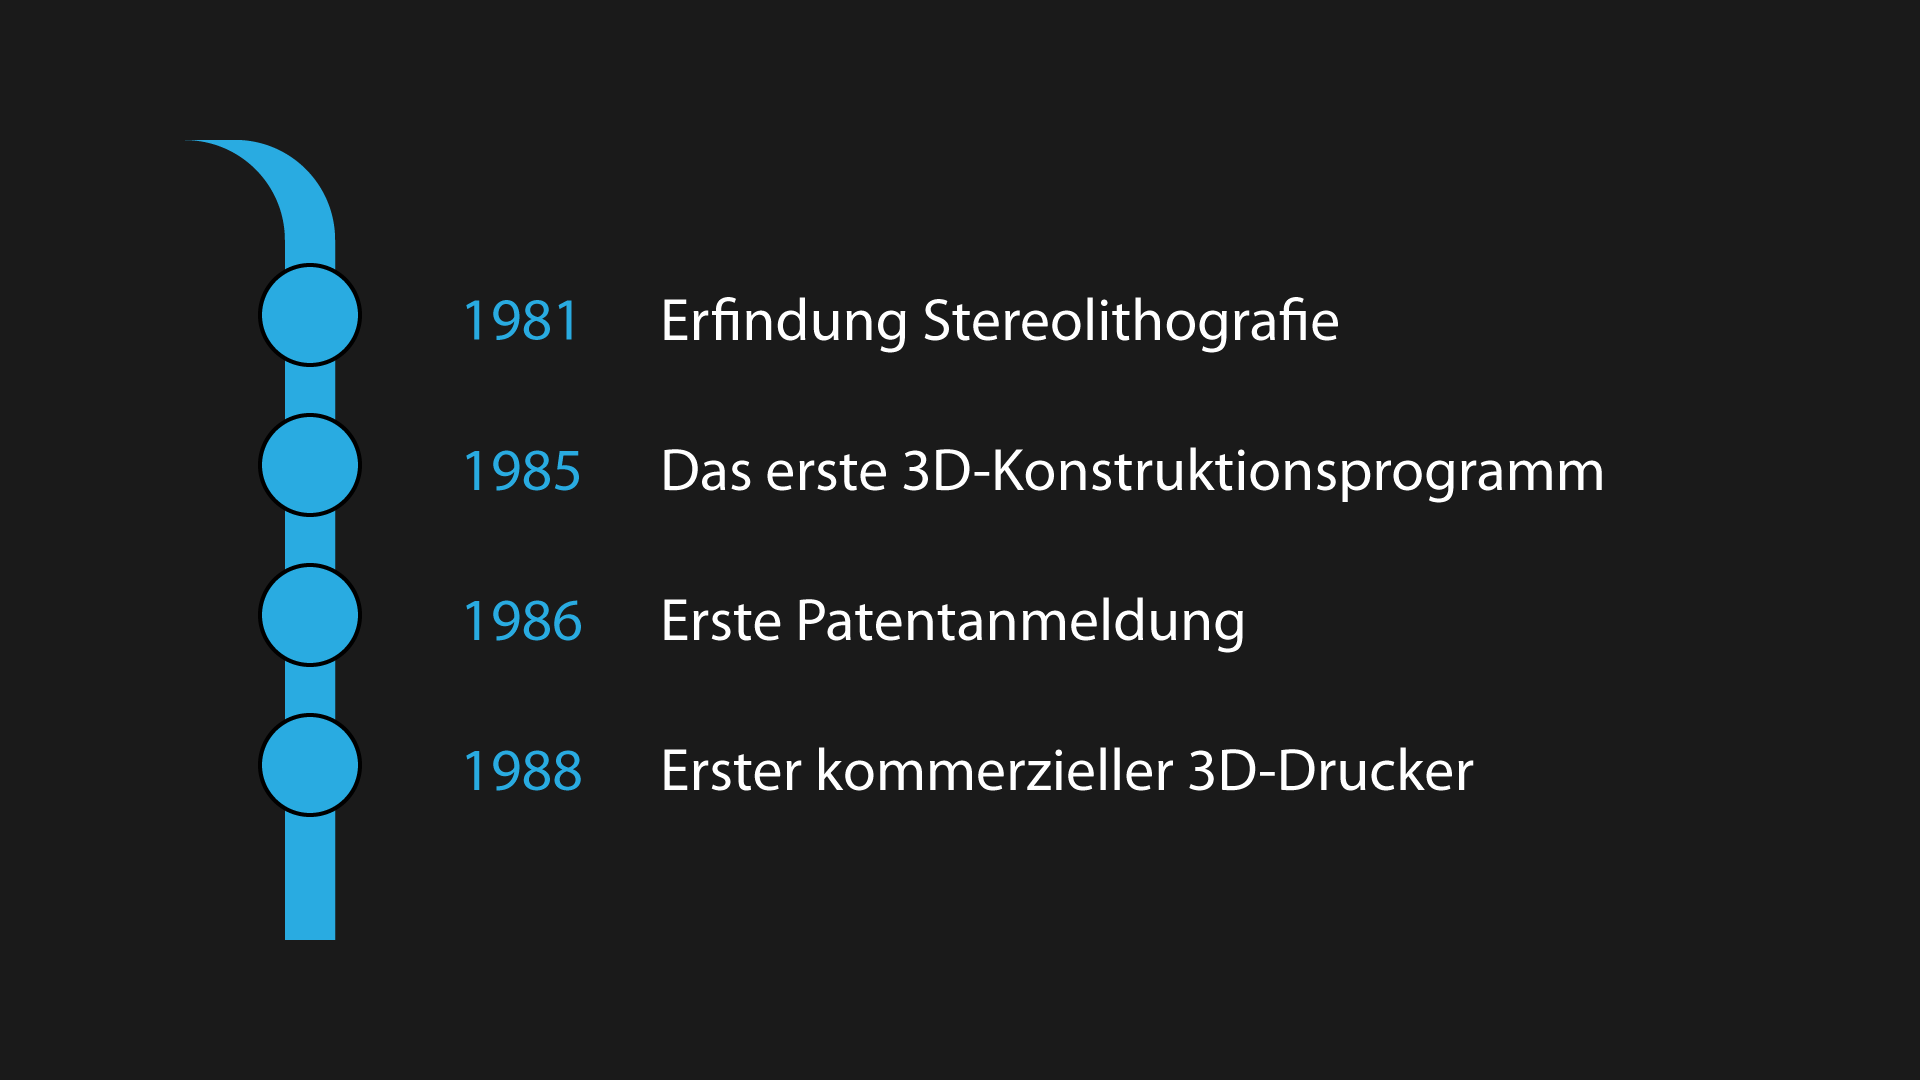
\includegraphics[width=1\paperwidth,height=1\paperheight,keepaspectratio]{images/geschichte/1980.png}};%
%\end{tikzpicture}}
\begin{frame}
  \frametitle{Seit wann gibt es 3D-Drucker}
\end{frame}
{
\usebackgroundtemplate{%
\colorbox{BackgroundJGH}{%
\vbox to \paperheight{\vfil\hbox to \paperwidth{\hfil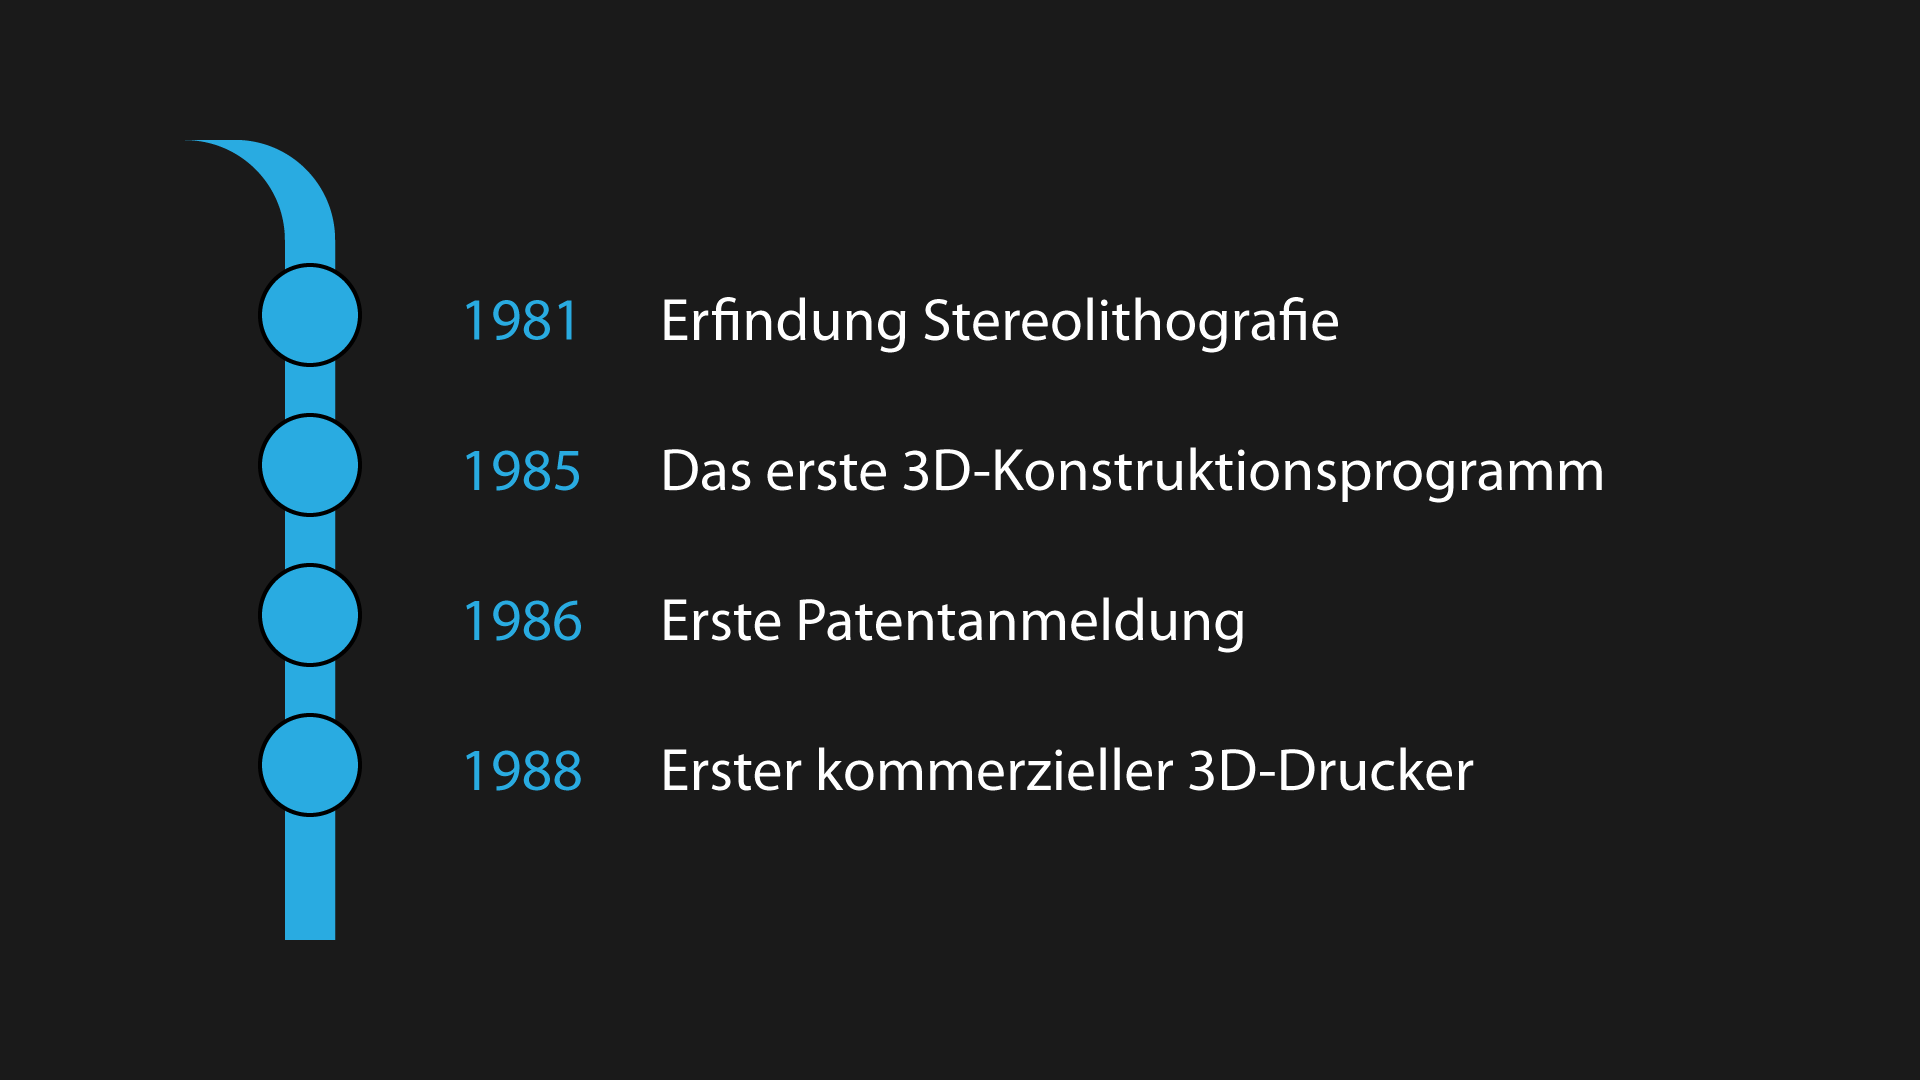
\includegraphics[width=\paperwidth]{images/geschichte/1980.png}\hfil}\vfil}
}
}
%\begin{tikzpicture}[background rectangle/.style={fill=olive!45},remember picture, overlay]%
%    \node at (current page.center) {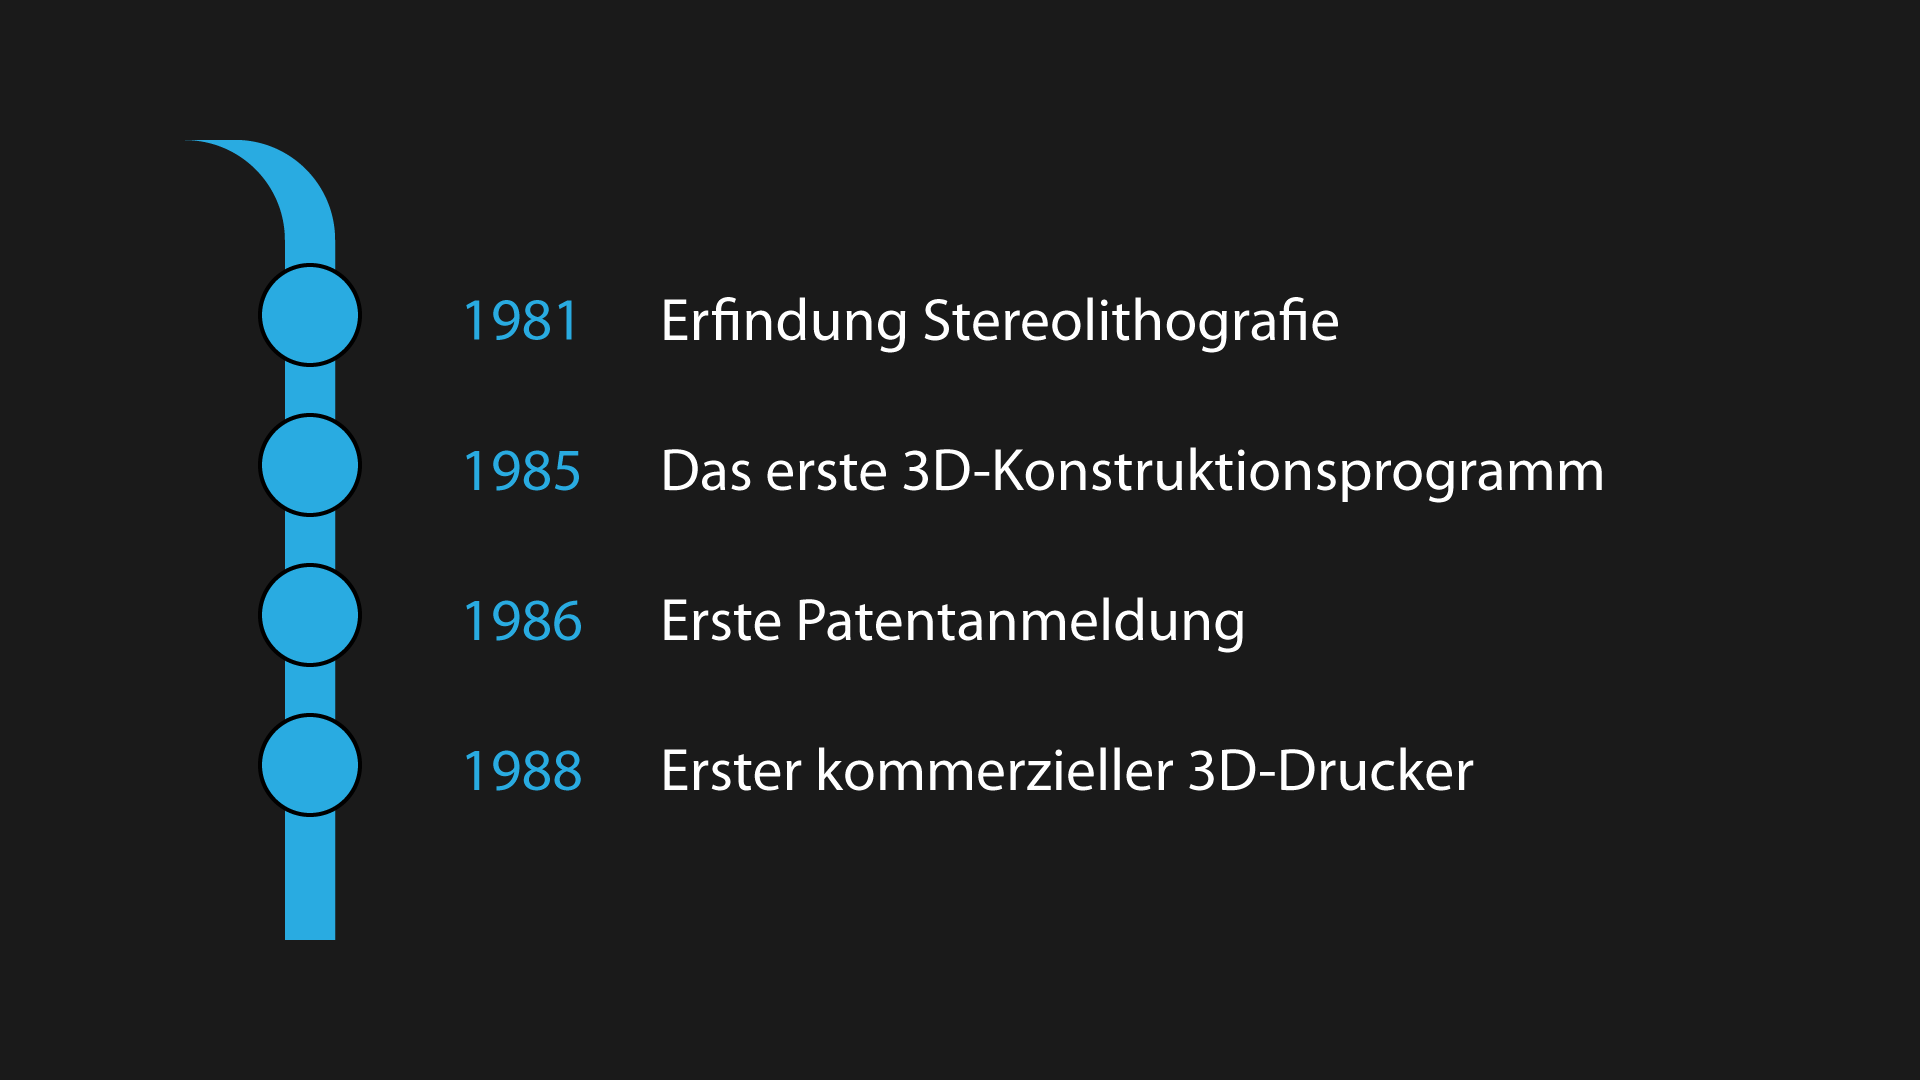
\includegraphics[width=1\paperwidth,height=1\paperheight,keepaspectratio]{images/geschichte/1980.png}};%
%\end{tikzpicture}}
\begin{frame}
  \frametitle{Seit wann gibt es 3D-Drucker}
\end{frame}
}
{
\usebackgroundtemplate{%
\colorbox{BackgroundJGH}{%
\vbox to \paperheight{\vfil\hbox to \paperwidth{\hfil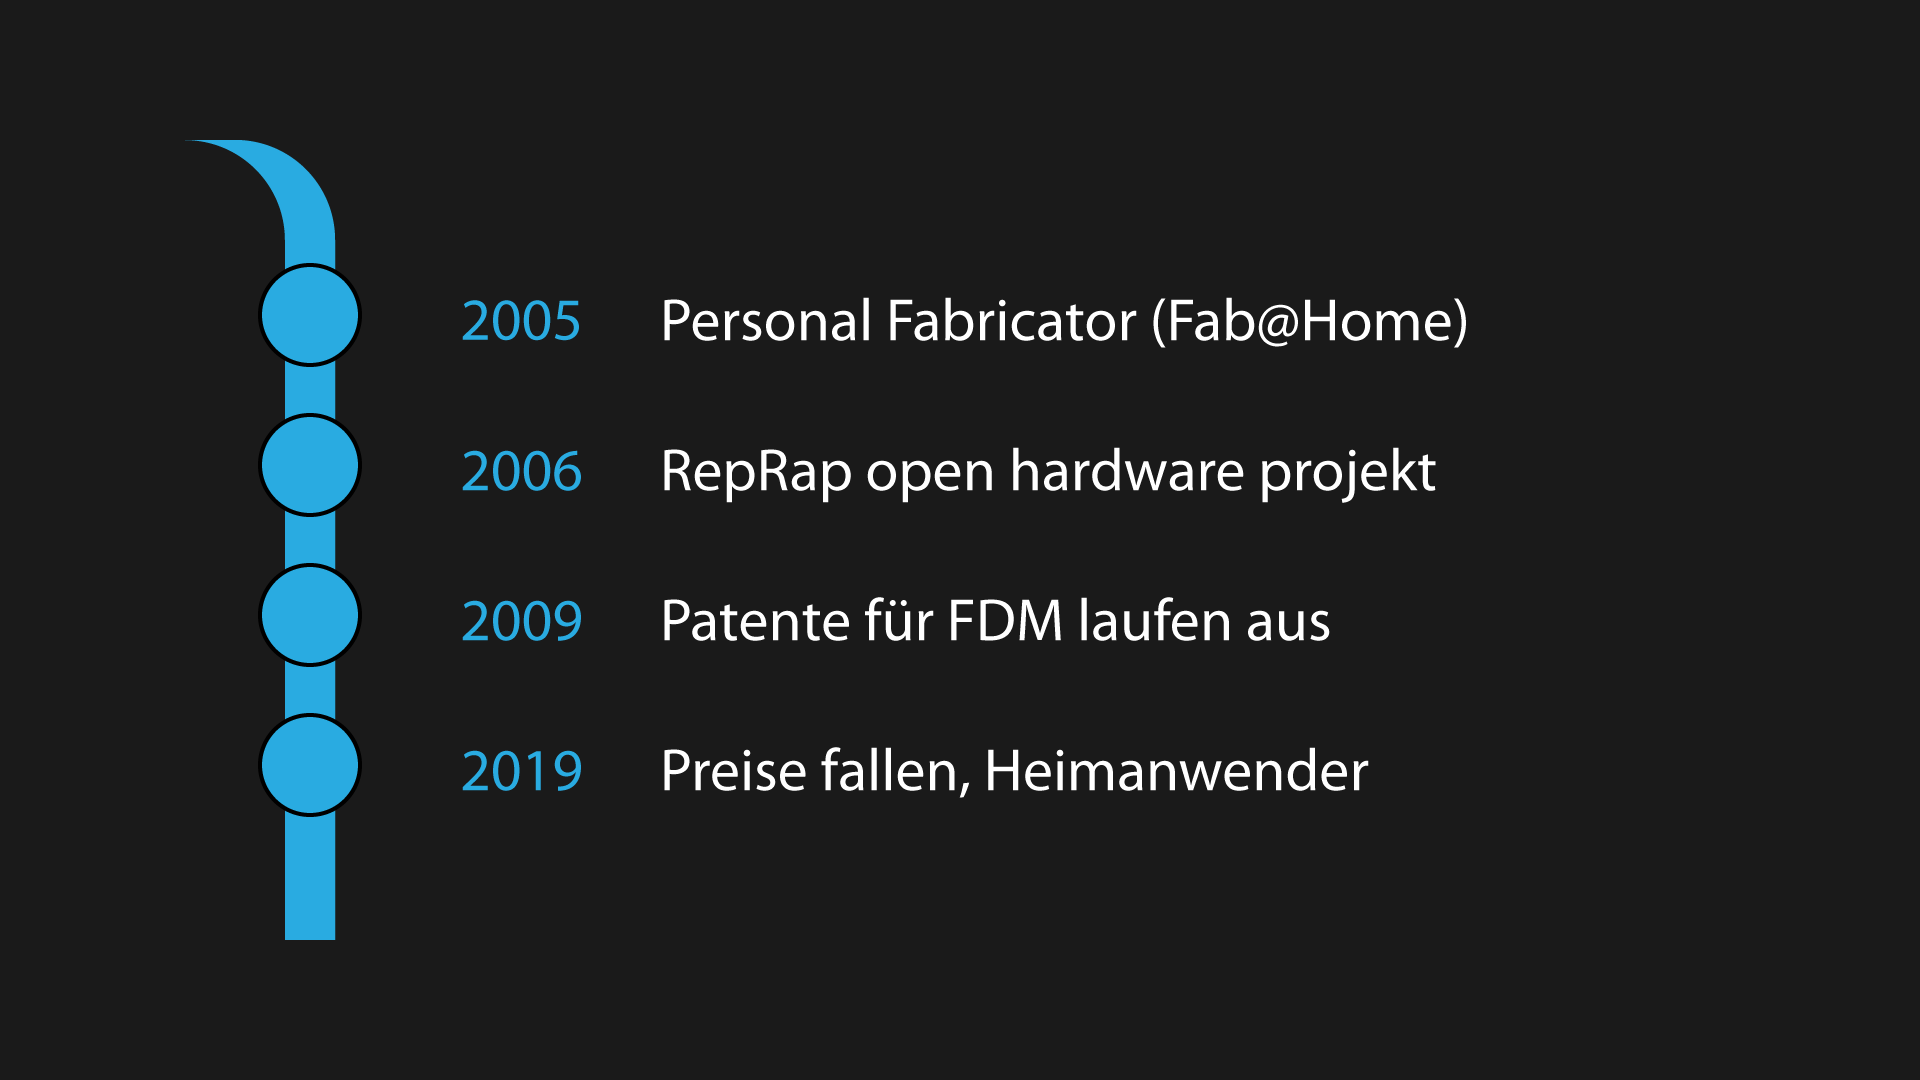
\includegraphics[width=\paperwidth]{images/geschichte/2000.png}\hfil}\vfil}
}
}
\begin{frame}
  \frametitle{Seit wann gibt es 3D-Drucker}
\end{frame}
}
